\documentclass{standalone}
\usepackage{graphicx}	
\usepackage{amssymb, amsmath}
\usepackage{color}

\usepackage{tikz}
\usetikzlibrary{intersections, backgrounds, math}
\usepackage{pgfmath}

\definecolor{light}{RGB}{220, 188, 188}
\definecolor{mid}{RGB}{185, 124, 124}
\definecolor{dark}{RGB}{143, 39, 39}
\definecolor{highlight}{RGB}{180, 31, 180}
\definecolor{lightteal}{RGB}{186, 219, 219}
\definecolor{midteal}{RGB}{124, 186, 186}
\definecolor{darkteal}{RGB}{38, 142, 142}
\definecolor{darkerteal}{RGB}{0, 124, 124}
\definecolor{gray10}{gray}{0.1}
\definecolor{gray20}{gray}{0.2}
\definecolor{gray30}{gray}{0.3}
\definecolor{gray40}{gray}{0.4}
\definecolor{gray60}{gray}{0.6}
\definecolor{gray70}{gray}{0.7}
\definecolor{gray80}{gray}{0.8}
\definecolor{gray90}{gray}{0.9}
\definecolor{gray95}{gray}{0.95}

\begin{document}

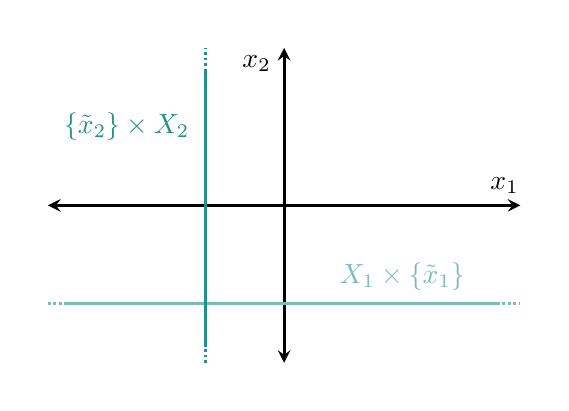
\begin{tikzpicture}[scale=1.0]

  \pgfmathsetmacro{\ys}{3.95};

  \draw[white] (-3.25, -2.25) rectangle (3.25, 2.25);
  
  \draw [<->, >=stealth, line width=1] (0, -2) -- +(0, 4);
  \draw [<->, >=stealth, line width=1] (-3, 0) -- +(6, 0);
  
  \node at (2.8, 0.25) { $x_{1}$ };
  \node at (-0.35, 1.8) { $x_{2}$ };
  
  \node[midteal] at (1.5, -0.9) { $ X_{1} \times \{ \tilde{x}_{1} \} $ };
  \draw[midteal, line width=1] (-2.8, -1.25) -- (2.7, -1.25);
  \draw[midteal, densely dotted, line width=1] (-3, -1.25) -- (-2.8, -1.25);
  \draw[midteal, densely dotted, line width=1] (2.7, -1.25) -- (3, -1.25);
    
  \node[darkteal] at (-2, 1) { $ \{ \tilde{x}_{2} \} \times X_{2} $ };
  \draw[darkteal, line width=1] (-1, -1.8) rectangle (-1, 1.7);
  \draw[darkteal, densely dotted, line width=1] (-1, -2) -- (-1, -1.8);
  \draw[darkteal, densely dotted, line width=1] (-1, 1.7) -- (-1, 2);
      
\end{tikzpicture}

\end{document}  